% section
\section{Introduction} \label{section::introduction}
 The thesis will compare different state-of-the-art solutions for image-/video-prediction \ref{subsection::imageprediction}.
 The main module of the solutions, which is the core aspect of this work, is the LSTM (Long short-term memory). \ref{subsection::lstm}.
 This module was invented by Hochreiter and Schmidhuber  \cite{Hochreiter1997} in 1997 and is used heavily in the field of image-\& video-prediction since then, e.g. in Srivastava et. al. 
 \cite{Srivastava2015}.
 During the time the module got many different add-ons and changes, which are described in different papers (\cite{Patraucean2015}, \cite{Lotter2016}, \cite{Wang2017}, \cite{Wang2018} and many 
 more.). To have a valid comparison, I implement three different state-of-the-art solutions for image-/video-prediction (\cite{Shi2015}, \cite{Patraucean2015} and \cite{Lotter2016}).
 All of them use the Shi et. al. ConvLSTM \cite{Shi2015} (Or a slightly different version) as recurrent sub-module, which is changed during the experiments
 with another, more advanced solution named PredRNN \cite{Wang2017}. The algorithms are re-implemented in PyTorch \cite{Paszke2019}, as well as the \glqq standard\grqq ConvLSTM and PredRNN.
 This introduction will cover the basic knowledge, the reader should have to follow the rest of the thesis.
 
 % subsection
 \subsection{Deep Learning} \label{subsection::deeplearning}
 
 % subsection
 \subsection{Backpropagation} \label{subsection::backpropagation}
 
 % subsection
 \subsection{Backpropagation through time (BPTT)} \label{subsection::bptt}
 
 % subsection
 \subsection{Image Prediction / Video Prediction} \label{subsection::imageprediction}
  Image-/Video-prediction is a field inside machine learning, where the key is to predict future images, given a sequence of image. The image sequence $X$ is of length $n$, ($x_0, \ldots, x_{n-1}$).
  One possible use-case is the one-frame prediction, where one predicts $x_n$, given the the sequence $X$. Another common use-case is multi-frame prediction, where the key is to predict $t$ many
  frames into the future. This is often performed using sequence-to-sequence learning \cite{Sutskever2014}. Obviously the first frames look much better then the last frames, as ground-truth is 
  missing, and the predicted frames are only approximated, which means they contain a certain level of error.

 % subsection
 \subsection{Autoencoder} \label{subsection::autoencoder}
  The autoencoder is a network architecture, which simply consists of two neural networks chained together. The first network is called \glqq Encoder\grqq. This part gets the input $x$ and outputs
  the \glqq code\grqq h. Often the output layer of the \glqq Encoder\grqq is named bottleneck-layer. The second network is called \glqq Decoder\grqq. It gets the \glqq code\grqq $h$ as input
  and outputs $\hat{x}$. This architecture is often used for reconstruction, where $x = \hat{x}$. To prevent the architecture to simply copy the input directly to the output (which would be an
  interpolation, and not the goal of an autoencoder.), there are different techniques to have the autoencoder to instead approximate the output, given the \glqq code\grqq h.
  The simplest autoencoder architecture is the so named \glqq undercomplete\grqq; autoencoder \cite{Goodfellow2016}, in which the output of the bottleneck-layer $h$ is smaller then the input $x$.
  Therefore the architecture needs to learn how to extract useful features from the input $x$, because it is not able to simply copy the input $x$ to the output $\hat{x}$. There are many different
  ideas of using an autoencoder architecture, which are described more in-depth in Goodfellow et. al. \cite{Goodfellow2016}.
  \begin{figure}[H]
   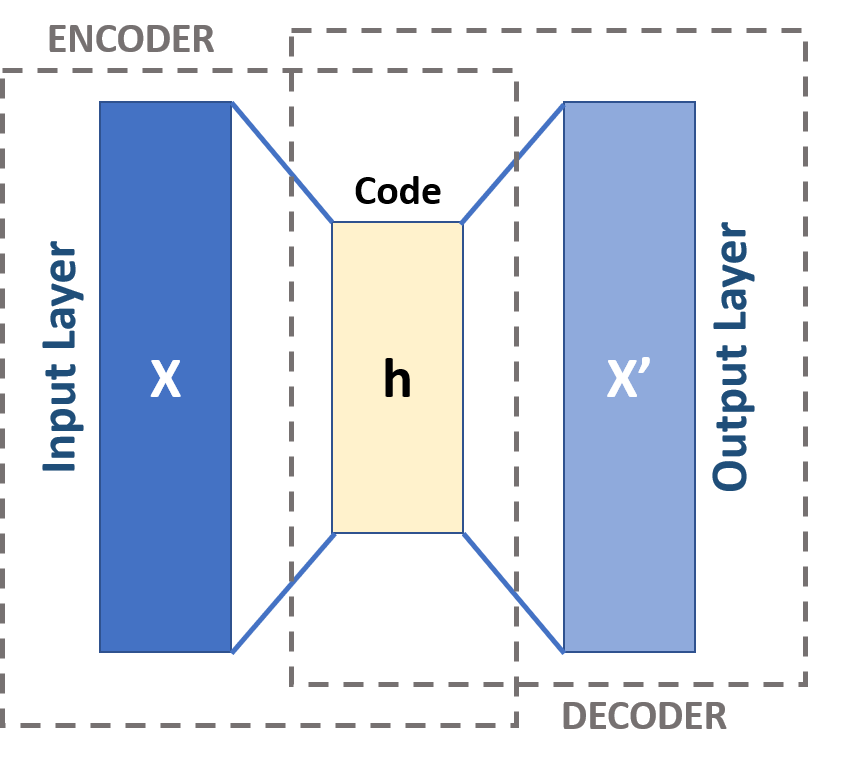
\includegraphics[width=0.4\textwidth]{../Images/autoencoder_schema.png}
   \centering
   \caption{Autoencoder schema \citep{wiki2019}}
   \label{fig:lstm_architecture}
  \end{figure}

 % subsection
 \subsection{RNN} \label{subsection::rnn}
  RNN (Recurrent neural network)
 
 % subsection
 \subsection{LSTM} \label{subsection::lstm}
  LSTM (Long Short-term Memory) \cite{Hochreiter1997} is a form of RNN, which avoids a critical problem of standard RNN: Saving \textbf{Long-term dependencies} \cite{Goodfellow2016}.
  The architecture consists of different submodules, an inpute-gate, forget-gate, cell-state and output-gate.
  \begin{equation}
   i_t = \sigma(w_{x_i}x_t + w_{h_i}h_{t-1} + w_{c_i}c_{t-1} + b_i)
  \end{equation}
  \begin{equation}
   f_t = \sigma(w_{x_f}x_t + w_{h_f}h_{t-1} + w_{c_f}c_{t-1} + b_f)
  \end{equation}
  \begin{equation}
   c_t = f_tc_{t-1} + i_ttanh(w_{x_c}x_t + w_{h_c}h_{t-1} + b_c)
  \end{equation}
  \begin{equation}
   o_t = \sigma(w_{x_o}x_t + w_{h_o}h_{t-1} + w_{c_o}c_t + b_o)
  \end{equation}
  \begin{equation}
   h_t = o_ttanh(c_t)
  \end{equation}
  $w$ is the weight of the layer, $\sigma$ the sigmoid function, $b$ the layer bias. $h_t$ is the output, in RNN's
  the output is often denoted as hidden.
  \begin{figure}[H]
   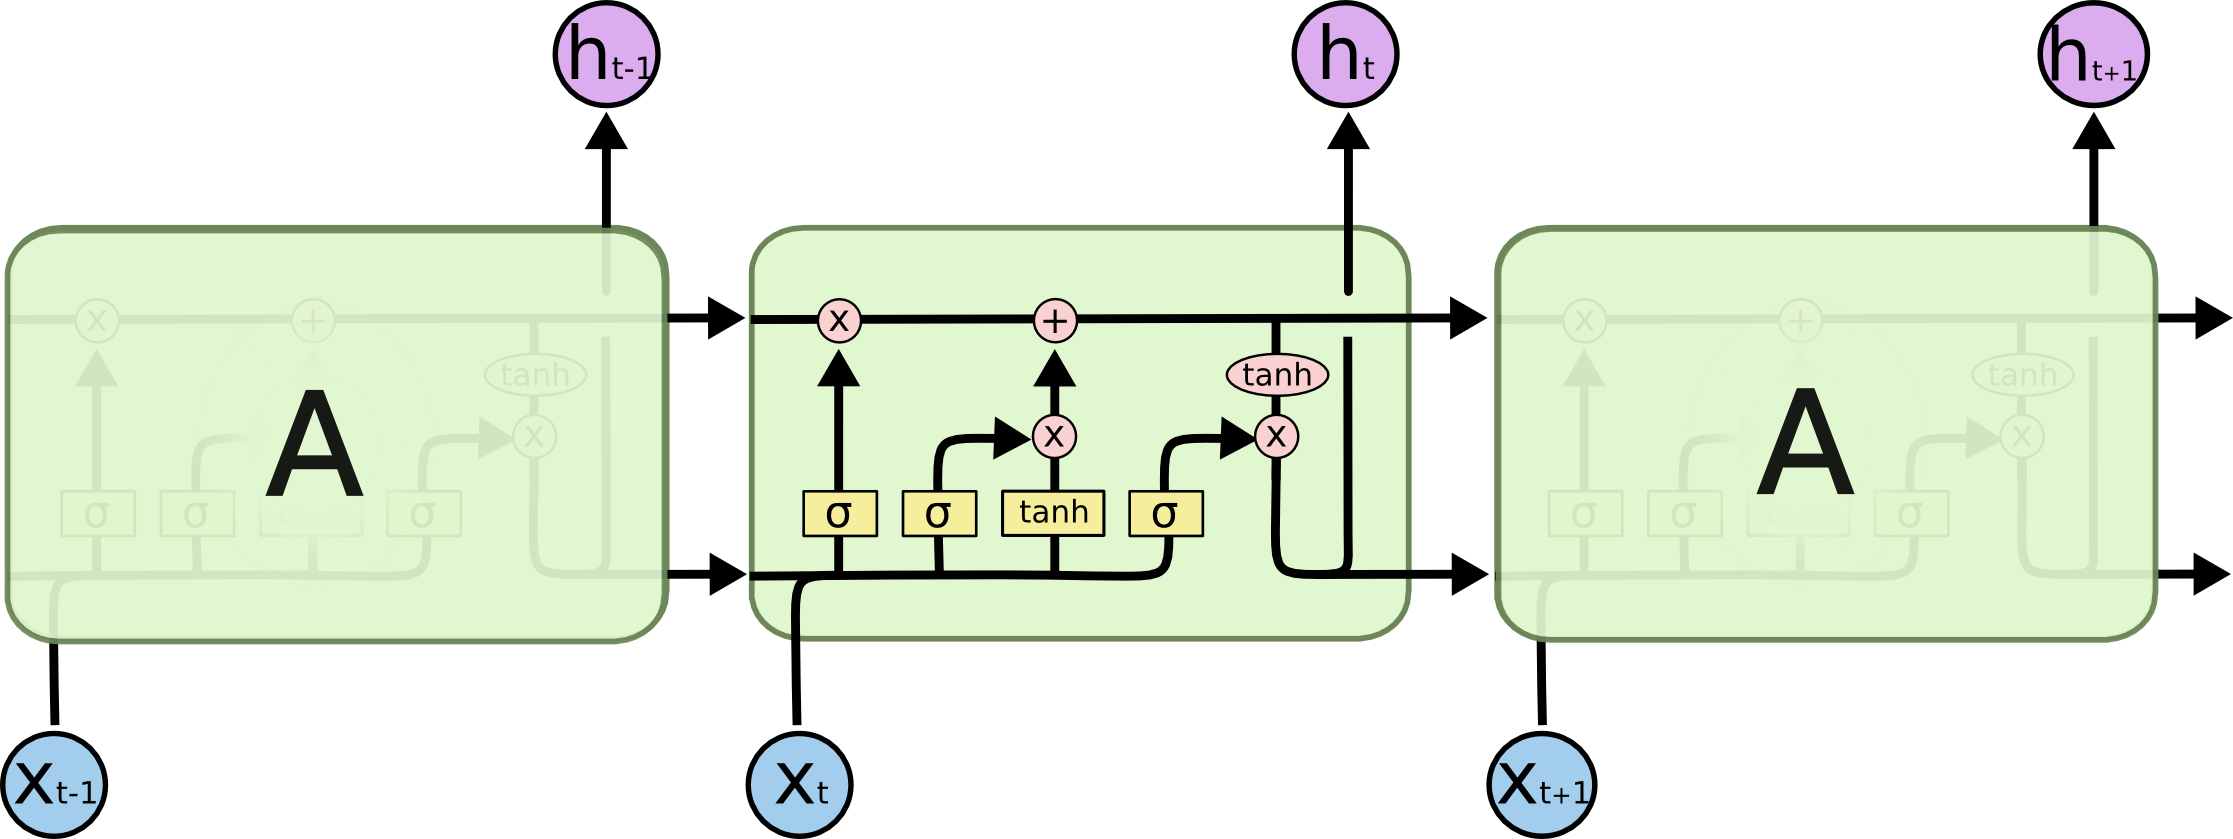
\includegraphics[width=0.6\textwidth]{../Images/lstm_chain.png}
   \centering
   \caption{LSTM Architecture \citep{Olah2015}}
   \label{fig:lstm_architecture}
  \end{figure}
 
 % subsection
 \subsection{ConvLSTM} \label{subsection::convlstm}
  The convolutional LSTM, invented by Shi et. al. \cite{Shi2015} is a LSTM using convolutional layer instead of fully connected ones. Therefore the formulas looks very similar to the ones in    
  section~\ref{subsection::lstm}.
  \begin{equation}
   i_t = \sigma(x_t \ast w_{x_i} + h_{t-1} \ast w_{h_i} + w_{i_b})
  \end{equation}
  \begin{equation}
   f_t = \sigma(x_t \ast w_{x_f} + h_{t-1} \ast w_{h_f} + w_{f_b})
  \end{equation}
  \begin{equation}
   \tilde{c_t} = tanh(x_t \ast w_{x_{\tilde{c}}} + h_{t-1} \ast w_{h_{\tilde{c}}} + w_{c_{\tilde{b}}})
  \end{equation}
  \begin{equation}
   c_t = \tilde{c_t} \odot i_t + c_{t-1} \odot f_t
  \end{equation}
  \begin{equation}
   o_t = \sigma(x_t \ast w_{x_o} + h_{t-1} \ast w_{h_o} + w_{o_b})
  \end{equation}
  \begin{equation}
   h_t = o_t \odot tanh(c_t)
  \end{equation}
  $\ast$ is the commonly used sign for the convolution operation.\\
  $\odot$ is the hadamard product (point-wise multiplication).
  
 % subsection
 \subsection{PyTorch} \label{subsection::pytorch}